\documentclass[12pt]{article}
\usepackage[utf8]{inputenc}
\usepackage[spanish]{babel}
\usepackage{amsmath, amssymb}
\usepackage{listings}
\usepackage{xcolor}
\usepackage{caption}
\usepackage{graphicx}
\usepackage{hyperref}
\usepackage{titlesec}
\usepackage{fancyvrb}
\usepackage{float}
\usepackage{booktabs}


\definecolor{codegray}{gray}{0.95}
\definecolor{codered}{rgb}{0.6,0,0}
\definecolor{codegreen}{rgb}{0,0.6,0}
\definecolor{codeblue}{rgb}{0,0,0.6}

\lstdefinestyle{mystyle}{
	backgroundcolor=\color{codegray},
	commentstyle=\color{codegreen},
	keywordstyle=\color{codered},
	numberstyle=\tiny\color{codeblue},
	stringstyle=\color{codegreen},
	basicstyle=\ttfamily\footnotesize,
	breaklines=true,
	numbers=left,
	numbersep=5pt,
	frame=single,
	tabsize=4,
	language=Python
}


\lstset{style=mystyle}


\title{Simulación de Eventos Discretos: Algoritmos de Planificación de Procesos}
\author{Jabel Resendiz Aguirre}
\date{Abril 2025}

\begin{document}
	
	\maketitle
	
	\begin{abstract}
		
	\end{abstract}
\section{Introducción al Planificador de la CPU}

El planificador de la CPU es una parte fundamental del sistema operativo de un sistema de computo ya que se encarga de decidir qué proceso va a utilizar la CPU en un momento determinado. 

El trabajo del planificador es seleccionar, de entre los procesos que están esperando para ejecutarse, cuál va a ser el siguiente en utilizar la CPU. Para hacerlo, el planificador sigue un conjunto de reglas, que se conocen como algoritmos de planificación. 

El planificador tiene un impacto directo en el rendimiento de la computadora. Su tarea no es sólo garantizar que todos los procesos se ejecuten, sino también hacerlo de manera que el sistema funcione de manera eficiente. Esto significa que el planificador debe minimizar el tiempo que los procesos pasan esperando y debe asegurarse de que los recursos de la CPU se utilicen de la mejor manera posible.

En este proyecto de simulación, nos enfocaremos en modelar el comportamiento de un sistema de planificación de CPU utilizando eventos discretos. La idea principal es analizar cómo los algoritmos de planificación, como el Round Robin, Multilevel Feedback Queue y SRTF impactan la ejecución de los procesos en un sistema con una única CPU. Para ello, simularemos cómo los procesos llegan al sistema y cómo son asignados a la CPU para su ejecución. Utilizaremos distribuciones probabilísticas, como la distribución exponencial y de Poisson, para modelar el tiempo entre llegadas de los procesos y sus tiempos de ejecución, lo que nos permitirá simular un entorno realista donde los tiempos de llegada y duración no son constantes, sino aleatorios.
 
\subsection{Características del sistema}
Para describir adecuadamente un sistema de colas, se deben tener en cuenta las siguientes características fundamentales:
 
 
 \begin{itemize}
 	\item \textbf{Patrón de llegada de los procesos:} Los procesos llegan al sistema siguiendo una distribución exponencial, lo que modela un proceso de Poisson. Esto representa un flujo aleatorio y continuo de solicitudes hacia la CPU, adecuado para entornos con alta incertidumbre en los tiempos de llegada.
 	
 	\item \textbf{Patrón de servicio del procesador:} El tiempo de CPU requerido por cada proceso se genera aleatoriamente usando distribuciones probabilísticas como la exponencial. Esto permite reflejar la variabilidad natural en la duración de las tareas reales.
 	
 	\item \textbf{Disciplina de cola:} Indica el orden en que los clientes son atendidos.En este proyecto se emplean reglas de secuenciación con prioridades, utilizando una técnica de planificación con desalojo (preemptive), en la cual el proceso que se encuentra en ejecución puede ser interrumpido para dar paso a otro de mayor prioridad dentro del sistema. Los algoritmos usados son: 
 	
 	\begin{itemize}
 		
 		\item \textbf{Round Robin (RR)}: Un algoritmo de planificación basado en asignar una cantidad fija de tiempo a cada proceso de manera cíclica.
 		
 		\item \textbf{Shortest Remaining Time First (SRTF)}: Un algoritmo de planificación preemptivo donde el proceso con el tiempo de ejecución restante más corto se ejecuta primero.
 		
 		\item \textbf{Multilevel Feedback Queue (MLFQ)}: Un algoritmo basado en múltiples colas con diferentes prioridades, donde los procesos son promovidos o degradados entre las colas según su comportamiento.
 		
 	\end{itemize}
 	
 	\item \textbf{Capacidad del sistema:} Es el número máximo de clientes que el sistema puede albergar, incluyendo los que están siendo atendidos y los que están esperando. Si la capacidad se supera, los nuevos clientes pueden ser rechazados o descartados.En nuestro sistema no estableceremos una cota para la cantidad de clientes (procesos), aunque eso no represente un escenario en sistemas embebidos o críticos donde sí hay un límite físico (RAM, threads u otros recursos propios).
 	 
 	\item \textbf{Número de canales de servicio:} Se refiere al número de servidores disponibles en paralelo. El modelo considera un sistema monoprocesador, donde existe un único canal de servicio (la CPU), encargado de ejecutar los procesos uno a uno según una disciplina de planificación preemptiva
 	
 	\item \textbf{Número de etapas de servicio:}  En nuestro caso, simulamos un sistema de planificación de CPU en el que cada proceso requiere únicamente una etapa de servicio: la ejecución en la CPU. No modelamos otras fases como entrada/salida (I/O) o espera por recursos externos . Por tanto, se trata de un sistema con una sola etapa de servicio.
 	
 \end{itemize}
	
\subsection{Objetivo y metas}

El objetivo principal de este proyecto es comprender y analizar el comportamiento de distintos algoritmos de planificación de CPU a través de una simulación estocástica de un sistema de colas. Adem\'as nos permite comparar la eficiencia de distintos algoritmos de planificación de CPU  evaluando métricas. Mediante la simulación y el análisis de estos algoritmos, buscamos entender mejor cómo las decisiones de planificación afectan el rendimiento global del sistema.

\subsection{Variables de interés }

\begin{itemize}
	\item \textbf{pid:} Identificador único para cada proceso. Se utiliza para hacer referencia y distinguir los diferentes procesos que entran al sistema.
	\item \textbf{arrival\_time:} Es el tiempo en el que un proceso llega al sistema, determinado por una distribución de llegadas.
	\item \textbf{burst\_time:} Tiempo de ejecución necesario para que el proceso complete su tarea. Esta variable es relevante para determinar cuánto tiempo se mantendrá el proceso ejecutándose en el CPU.
	\item \textbf{start\_time:} Es el momento en que un proceso comienza su ejecución en el procesador. Esta variable se establece más tarde, cuando el proceso es seleccionado por el planificador.
	\item \textbf{end\_time:} Es el tiempo cuando el proceso finaliza su ejecución. Al igual que el tiempo de inicio, este valor se calcula una vez que el proceso ha completado su tarea.
	\item \textbf{waiting\_time:} Es el tiempo que un proceso pasa esperando antes de que comience su ejecución. Se calcula como la diferencia entre el tiempo de vuelta y el tiempo de ejecución (\texttt{waiting\_time = turnaround\_time - burst\_time}).
	
	\item \textbf{turnaround\_time:} Es el tiempo total que transcurre desde la llegada de un proceso hasta su finalización. Se calcula como la diferencia entre el tiempo de finalización y el tiempo de llegada (\texttt{turnaround\_time = end\_time - arrival\_time}).
	
	\item \textbf{remaining\_time:} Indica el tiempo restante para completar la ejecución del proceso. Esta variable es especialmente útil en algoritmos preemptivos.
	
\end{itemize}

\subsection{Variables que describen el problema}
Como bien describimos en las caracteristicas de nuestro sistema , nuestras variables que describen el problema son :

\begin{itemize}
	\item \textbf{Patrón de llegada de los procesos:} El tiempo entre la llegada de los procesos se modela utilizando una distribución \textit{exponencial}, lo cual implica un proceso de \textit{Poisson}. Esto significa que los procesos llegan de manera aleatoria, y el tiempo entre llegadas sigue una distribución exponencial con una tasa promedio de llegada.
	
	\item \textbf{Patrón de servicio de los procesos:} El tiempo de ejecución de cada proceso (o tiempo de ráfaga) también se modela utilizando una distribución \textit{exponencial}. Este tiempo de servicio determina cuánto tiempo cada proceso ocupará la CPU antes de completarse.
	
	\item \textbf{Número de procesos:} Este es el número total de procesos que el sistema debe manejar durante la simulación. Los procesos llegarán al sistema según el patrón de llegada descrito previamente.
	
	\item \textbf{Capacidad de la cola:} Este es el número máximo de procesos que pueden esperar en la cola de ejecución. En este proyecto no se establece una capacidad máxima para la cola, lo que permite que el sistema acepte y procese una cantidad arbitraria de procesos a lo largo de la simulación.
	
	\item \textbf{Número de canales de servicio:} El sistema tiene un solo canal de servicio, lo que significa que se utiliza un solo procesador de CPU para ejecutar los procesos. Este sistema se considera mono-servidor.
	
	\item \textbf{Disciplina de cola:} En este proyecto se implementan algoritmos de planificación de CPU como Round Robin,Multilevel Feedback Queue{MLFQ} o Shortest Remaining Time First (SRTF).
	
\end{itemize}


\section{Detalles de Implementación}

La simulación de planificación de procesos en CPU fue desarrollada en Python mediante un enfoque de eventos discretos. La arquitectura es modular y extensible, permitiendo simular múltiples algoritmos. A continuación se detallan los elementos principales:

\begin{itemize}
	
	\item \textbf{Estructuras principales:} Se definieron las clases \texttt{Process} y \texttt{Event} para representar procesos y eventos respectivamente.
	
	\begin{lstlisting}[language=Python, caption={Clase Process}]
		class Process:
		def __init__(self, pid, arrival, duration):
			self.pid = pid
			class Process:
			def __init__(self, pid, arrival_time, burst_time):
			self.pid = pid                      # Unique identifier for each process
			self.arrival_time = arrival_time    # Time when the process arrives
			self.burst_time = burst_time        # Execution time of the process
			self.start_time = None              # Time when the process starts executing (to be set later)
			...
			
	\end{lstlisting}
	
	\begin{lstlisting}[language=Python, caption={Clase Event}]
		class Event:
			def __init__(self, time, event_type, process):
				self.time = time                    # Time when this event occurs
				self.event_type = event_type        # Type of the event (e.g., 'arrival', 'completion')
				self.process = process              # The process involved in the event
		
			def __lt__(self, other):
				"""Defines how to compare events"""
				return self.time < other.time
		
		
	\end{lstlisting}
	
	\item \textbf{Interfaz para los planificadores:} Se definió una interfaz \texttt{IScheduling}, que estandariza los métodos que todo algoritmo de planificación debe implementar, como el manejo de llegadas, finalización y ejecución de procesos. Esto facilita la extensibilidad del simulador.
	
	\begin{lstlisting}[language=Python, caption={Interfaz IScheduling}]
		class IScheduling(ABC):
			@abstractmethod
			def add_process(self, process): pass
		
			@abstractmethod
			def process_event(self, event): pass
	\end{lstlisting}
	
	\item \textbf{Cola de eventos:} Se utilizó una \textit{priority queue} (cola de prioridad) para almacenar eventos, ordenados por tiempo de llegada, es la forma que tiene el algoritmo de saber el orden en que llegan los procesos.
	
	\begin{lstlisting}[language=Python, caption={Cola de eventos con heapq}]
		import heapq
		
		def add_process(self, process: Process):
		self.processes.append(process)
		arrival_event = Event(process.arrival_time, 'ARRIVAL', process)
		heapq.heappush(self.event_queue, arrival_event)
		
	\end{lstlisting}
	
	\item \textbf{Algoritmos de planificación:} Cada algoritmo está encapsulado en una clase que implementa una interfaz común. Se implementaron FCFS, SRTF, Round Robin y MLFQ.
	
	\begin{lstlisting}[language=Python, caption={Ejemplo de Round Robin}]
		class RoundRobin(IScheduling):
		def __init__(self, quantum):
			super().__init__()
			self.quantum = quantum
			self.ready_queue = deque()
			self.running_process = None  
			
			
	\end{lstlisting}
	
	\item \textbf{Preempción:} En los algoritmos como SRTF o MLFQ, se implementa lógica para interrumpir el proceso actual si uno de mayor prioridad llega. Para ellos se usan colas con prioridad para ir manteniendo la prioridad entre los procesos que ya han sido generados hasta ese momento.
	
	\item \textbf{Cálculo de métricas:} Se calcularon métricas como el tiempo promedio de espera y de retorno al finalizar todos los procesos.
	
	\begin{lstlisting}[language=Python, caption={Tiempo de espera promedio}]
		def statistics(self):
			results = {}
			for scheduler_name, scheduler in [
				("MLFQ", self.mlfq_scheduler),
				("RoundRobin", self.round_robin_scheduler),
				("SRTF", self.srtf_scheduler)
			]:
				turnaround = [p.turnaround_time for p in scheduler.completed_processes]
				waiting = [p.waiting_time for p in scheduler.completed_processes]
				results[scheduler_name] = {
						'avg_turnaround_time': np.mean(turnaround) if turnaround else 0,
						'avg_waiting_time': np.mean(waiting) if waiting else 0,
						'processes': len(scheduler.completed_processes)
										}
			return results
	\end{lstlisting}
	
	\item \textbf{Pruebas y validación:} Se ejecutaron pruebas con parámetros aleatorios, distribuciones controladas y se compararon resultados entre algoritmos.
	
	
\end{itemize}

\subsection{Funcionamiento de mi Simulaci\'on}:

\begin{itemize}
	\item Se definen mis variables del problema utilizadas para calcular los tiempos de arribo y el tiempo que necesita la CPU para completar cada proceso. As\'i como tambi\'en se sabe el tiempo de estudio de la simulaci\'on.
	\item Se procesan los datos de todos los procesos de mi simulaci\'on teniendo en cuenta que en nuestra definici\'on los procesos son independientes. 
	\item Se ejecutan los algoritmos definidos previamente ,uno a la vez con la misma lista de procesos previos definidos
	\item Se recoge y recopila informaci\'on del estado y la vida de cada proceso en un algoritmo y se muestra , listo para ser procesados
	\item Se interpretan los datos obtenidos apoy\'andonos de gr\'aficos y tablas.
	\item Se ejecutan pruebas con parámetros aleatorios, distribuciones controladas y se comparan resultados entre algoritmos.
	
\end{itemize}

	
	
	
	
	
	
	
	
	
	\section{Resultados y Experimentos}
	
En esta sección, se presentan los resultados obtenidos a partir de la simulación de algoritmos de planificación de CPU, específicamente utilizando el algoritmo \texttt{SRTF}. El objetivo es evaluar el rendimiento de este algoritmo bajo diferentes condiciones de carga. Los experimentos se diseñaron con el fin de analizar cómo varían las métricas de rendimiento a medida que se cambian parámetros clave del sistema.

\subsection{Configuración de los Experimentos}

La simulación fue configurada con los siguientes parámetros clave:


\begin{itemize}
	\item \textbf{Tasa de llegada de procesos (\(\lambda\))}: Representa el número promedio de procesos que llegan al sistema por unidad de tiempo. En este caso, se evaluaron tres valores de \(\lambda\), que corresponden a diferentes niveles de carga: 0.3, 0.7 y 0.9.
	\item \textbf{Tasa de ejecución (\(\mu\))}: Se mantuvo constante en 1.0, lo que indica que los procesos se ejecutan a una tasa fija.
	\item \textbf{Tiempo de simulación}: Se definió un tiempo de cierre de 1000 unidades de tiempo, durante el cual se realiza el proceso de simulación.
	\item \textbf{Número de réplicas}: Para cada configuración de parámetros, se realizaron 200 réplicas para asegurar la robustez estadística de los resultados obtenidos, esto se hace para reducir al varianza y obtener estimaciones mas confiables de las metricas de rendimiento
\end{itemize}

\subsection{Ejecución de la Simulación}

La simulación se ejecutó para cada uno de los valores de \(\lambda\). Para cada réplica:
\begin{itemize}
	\item Se creó una nueva instancia de la simulación con el valor de \(\lambda\), manteniendo constante \(\mu\) y el tiempo de simulación.
	\item Se ejecutaron los eventos correspondientes para modelar el comportamiento del algoritmo de planificación de CPU (\texttt{SJFB} en este caso).
	\item Al finalizar cada ejecución, se recolectaron las estadísticas de rendimiento.
\end{itemize}


\subsection{Experimentos Realizados:}

A continuación se describen los experimentos realizados para evaluar el efecto de la tasa de llegada de procesos (\(\lambda\)) sobre el rendimiento del sistema.

\subsubsection{Efecto de la tasa de llegada (\(\lambda\)) sobre el tiempo de espera promedio}

\textbf{Objetivo:} Observar cómo el tiempo de espera promedio aumenta o disminuye conforme se incrementa la tasa de llegada (\(\lambda\)).

\textbf{Hipótesis:} A medida que \(\lambda\) aumenta, los procesos llegan más rápido, lo que provoca mayores tiempos de espera debido a la congestión en la cola. 

\textbf{Métrica:} Tiempo de espera promedio (\texttt{avg\_waiting\_time}).

\textbf{Experimento:} Para este experimento, se varió \(\lambda\) en tres niveles: 0.3, 0.7 y 0.9. Se ejecutaron 200 réplicas para cada valor de \(\lambda\), y se observó cómo el tiempo de espera promedio se comportaba para cada uno de estos niveles. Los resultados fueron graficados con \(\lambda\) en el eje \(X\) y el tiempo de espera promedio en el eje \(Y\). Adem\'as utiliza intervalos de confianza del 95\% para mostrar la incertidumbre de los resultados.

\begin{figure}[H]
	\centering
	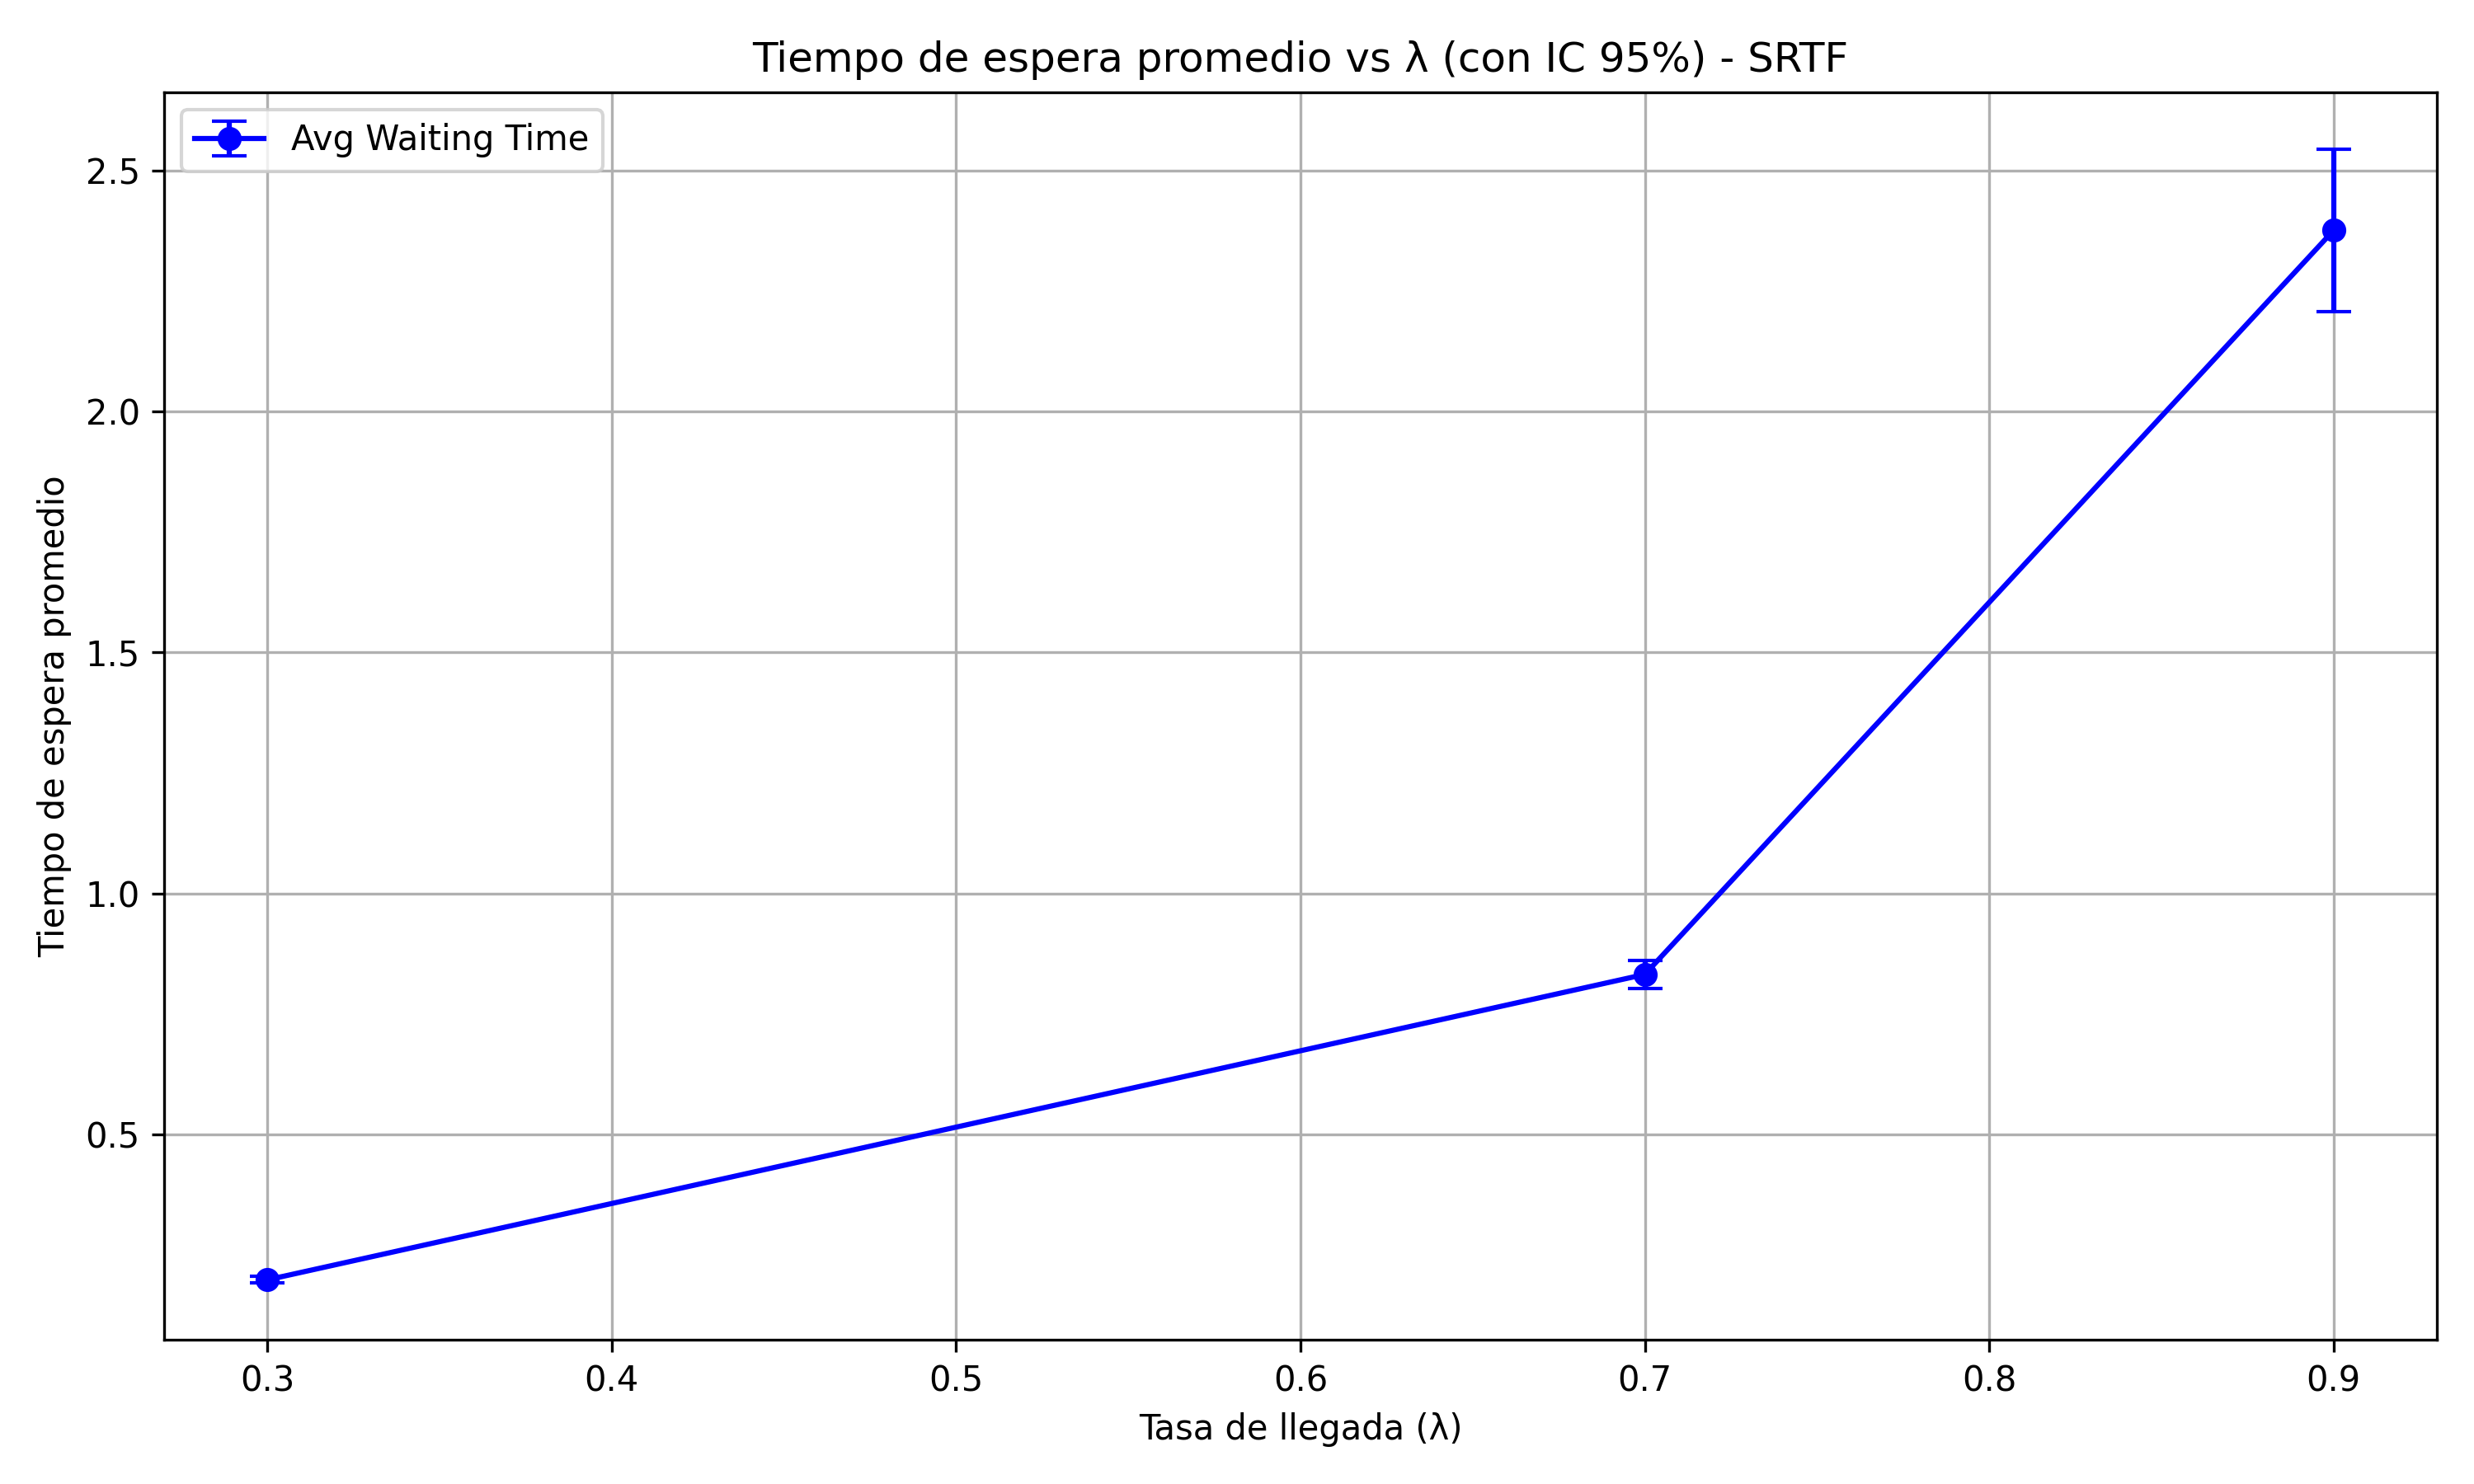
\includegraphics[width=0.8\textwidth]{tiempo_espera_vs_lambda.png}
	\caption{Tiempo de espera promedio vs tasa de llegada (\(\lambda\)) con intervalo de confianza del 95\%).}
	\label{fig:tiempo_espera_vs_lambda}
\end{figure}

El comportamiento esperado es que a medida que \(\lambda\) aumenta, el tiempo de espera promedio también aumentará debido a la mayor cantidad de procesos que llegan al sistema en menor tiempo.


En el gráfico de arriba, se muestra cómo el tiempo de espera promedio varía a medida que cambia la tasa de llegada. La línea muestra la media de los tiempos de espera, mientras que las barras de error indican el intervalo de confianza del 95\%.

Como se puede observar, el tiempo de espera promedio tiende a aumentar conforme aumenta la tasa de llegada \(\lambda\). Sin embargo, a medida que nos acercamos al valor crítico de \(\lambda \approx 1\), el crecimiento del tiempo de espera se acelera significativamente. Este comportamiento está relacionado con el concepto de \textbf{utilización del sistema} \(\rho\), que es una medida de la ocupación del CPU.

Matemáticamente, la utilización del sistema se define como:

\[
\rho = \frac{\lambda}{\mu}
\]

Donde:
- \(\lambda\) es la tasa de llegada de procesos.
- \(\mu\) es la tasa de servicio del sistema (en este caso, la tasa a la que el CPU procesa los procesos).

Cuando \(\rho\) se acerca a 1, es decir, cuando la tasa de llegada de procesos se acerca a la tasa de servicio, el sistema comienza a estar saturado, lo que genera una cola creciente de procesos esperando ser ejecutados. En términos prácticos, cuando \(\lambda\) se acerca a \(\mu\), la cola de procesos crece rápidamente, ya que el CPU está ocupado la mayor parte del tiempo, lo que incrementa el tiempo de espera de los procesos en la cola.

Este fenómeno es conocido como \textit{congestión} del sistema. Matemáticamente, la fórmula que describe el tiempo de espera promedio en un sistema M/M/1 (que es el tipo de sistema que estamos simulando) es la siguiente:

\[
W_q = \frac{\lambda}{\mu(\mu - \lambda)}
\]

Donde:
- \(W_q\) es el tiempo de espera promedio en la cola.
- \(\lambda\) es la tasa de llegada de procesos.
- \(\mu\) es la tasa de servicio del sistema.

Esta fórmula muestra que, conforme \(\lambda\) se acerca a \(\mu\), el tiempo de espera en la cola \(W_q\) crece de manera exponencial. Esto es consistente con los resultados observados en el gráfico, donde a medida que \(\lambda\) se aproxima a 1, el tiempo de espera promedio aumenta rápidamente debido a la saturación del sistema.


\subsubsection*{Efecto de la tasa de llegada (\(\lambda\)) sobre el tiempo de retorno promedio}

\textbf{Objetivo:} Evaluar cómo la tasa de llegada de procesos impacta el tiempo total que un proceso pasa en el sistema (tiempo de retorno).

\textbf{Hipótesis:} A medida que \(\lambda\) aumenta, los procesos tienden a acumularse en la cola del sistema, lo que provoca un incremento en el tiempo total desde la llegada hasta la finalización, es decir, en el tiempo de retorno.

\textbf{Métrica:} Tiempo de retorno promedio (\texttt{avg\_turnaround\_time}).

\textbf{Experimento:} Se varió \(\lambda\) en tres niveles: 0.3, 0.7 y 0.9, manteniendo constante la tasa de ejecución \(\mu = 1.0\). Para cada valor de \(\lambda\), se realizaron 200 réplicas, y se calculó el tiempo de retorno promedio.

A continuación, se muestra el gráfico correspondiente, donde se puede observar la relación entre \(\lambda\) y el tiempo de retorno promedio, incluyendo los intervalos de confianza al 95\%:

\begin{figure}[H]
	\centering
	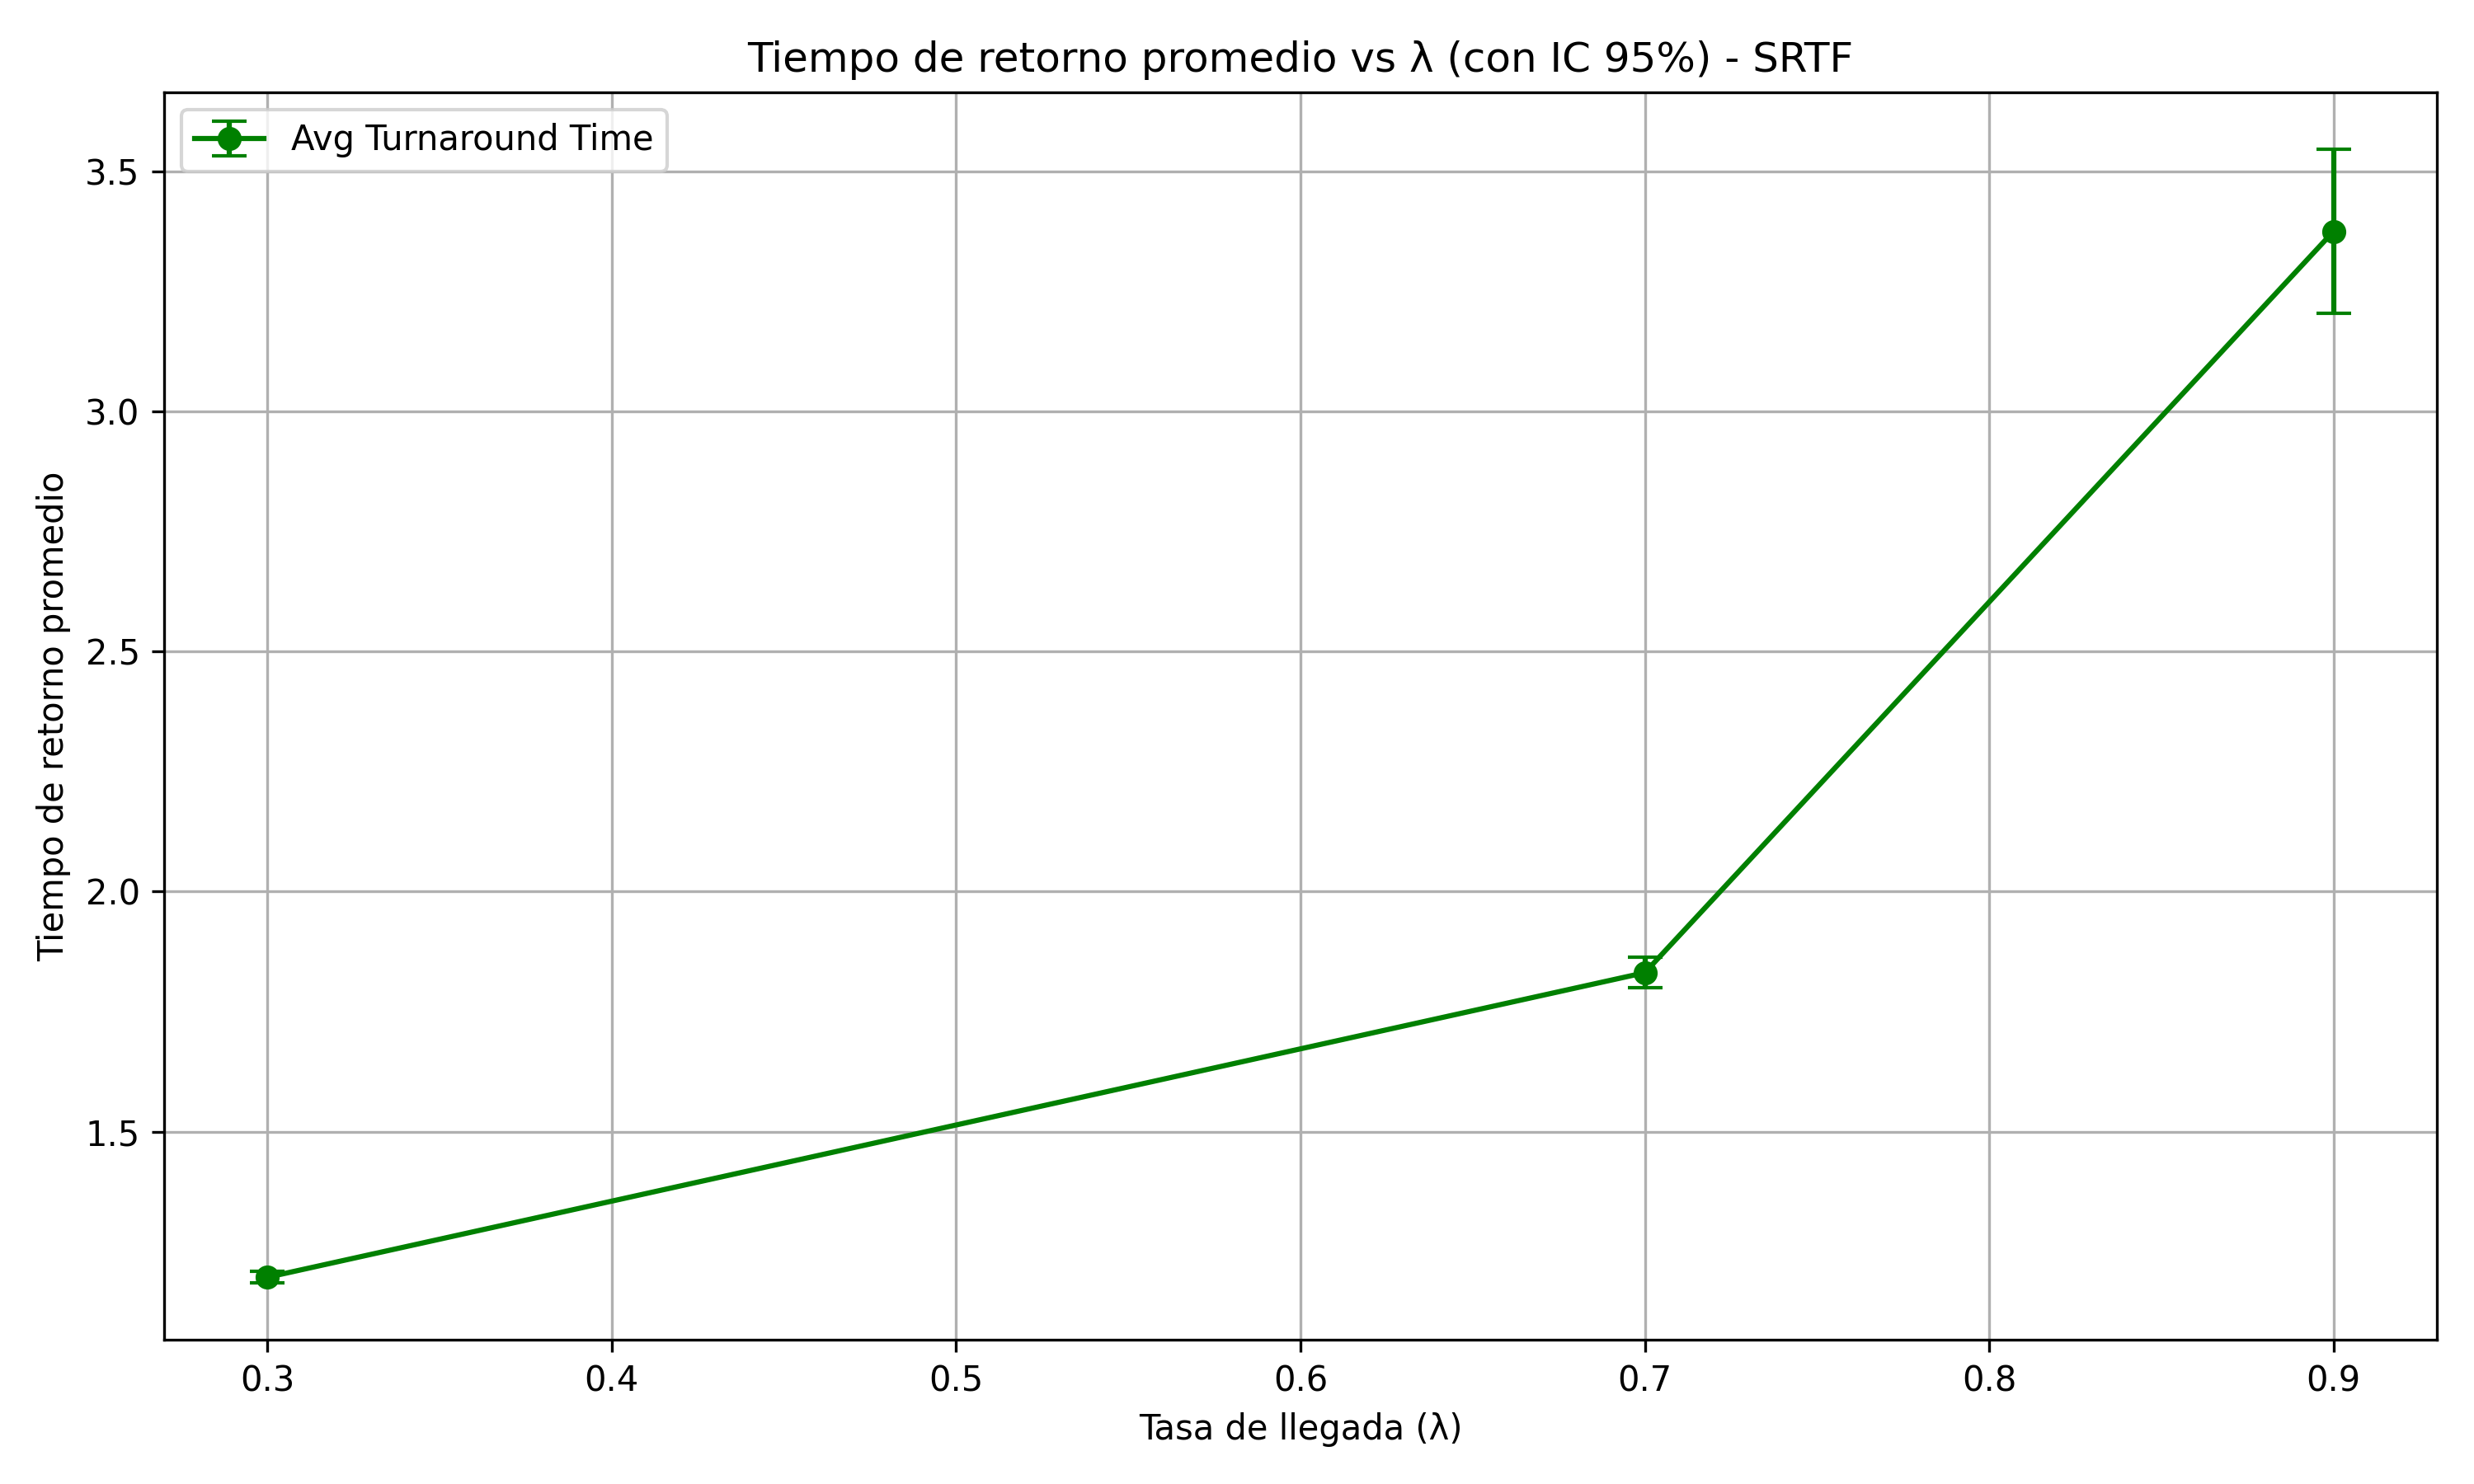
\includegraphics[width=0.75\textwidth]{tiempo_retorno_vs_lambda.png}
	\caption{Tiempo de retorno promedio vs tasa de llegada \(\lambda\) con IC 95\%}
	\label{fig:turnaround_vs_lambda}
\end{figure}

\textbf{Análisis adicional:} Al aumentar \(\lambda\), el sistema se aproxima a su límite de capacidad. Esto se refleja en la razón de utilización del servidor, \(\rho = \frac{\lambda}{\mu}\). A medida que \(\rho\) se acerca a 1, la congestión crece significativamente y las colas se hacen más largas, lo que genera un crecimiento acelerado tanto en el tiempo de espera como en el tiempo de retorno. Matemáticamente, en teoría de colas M/M/1, el tiempo promedio en el sistema está dado por:

\[
\mathbb{E}[T] = \frac{1}{\mu - \lambda}
\]

lo cual muestra que, conforme \(\lambda \to \mu\), el tiempo en el sistema tiende a infinito.



\subsubsection*{Efecto de la tasa de llegada (\(\lambda\)) sobre el tamaño de la cola promedio}

\textbf{Objetivo:} Evaluar cómo la tasa de llegada de procesos impacta el tamaño promedio de la cola en el sistema.

\textbf{Hipótesis:} A medida que \(\lambda\) aumenta, la probabilidad de que los procesos lleguen al sistema más rápidamente que la capacidad del servidor para procesarlos también aumenta, lo que provoca un incremento en el tamaño de la cola promedio.

\textbf{Métrica:} Tamaño de la cola promedio (\texttt{avg\_queue\_size}).

\textbf{Experimento:} Se varió \(\lambda\) en tres niveles: 0.3, 0.7 y 0.9, manteniendo constante la tasa de ejecución \(\mu = 1.0\). Para cada valor de \(\lambda\), se realizaron 200 réplicas y se calculó el tamaño promedio de la cola.

A continuación, se muestra el gráfico correspondiente, donde se puede observar la relación entre \(\lambda\) y el tamaño de la cola promedio, incluyendo los intervalos de confianza al 95\%:

\begin{figure}[H]
	\centering
	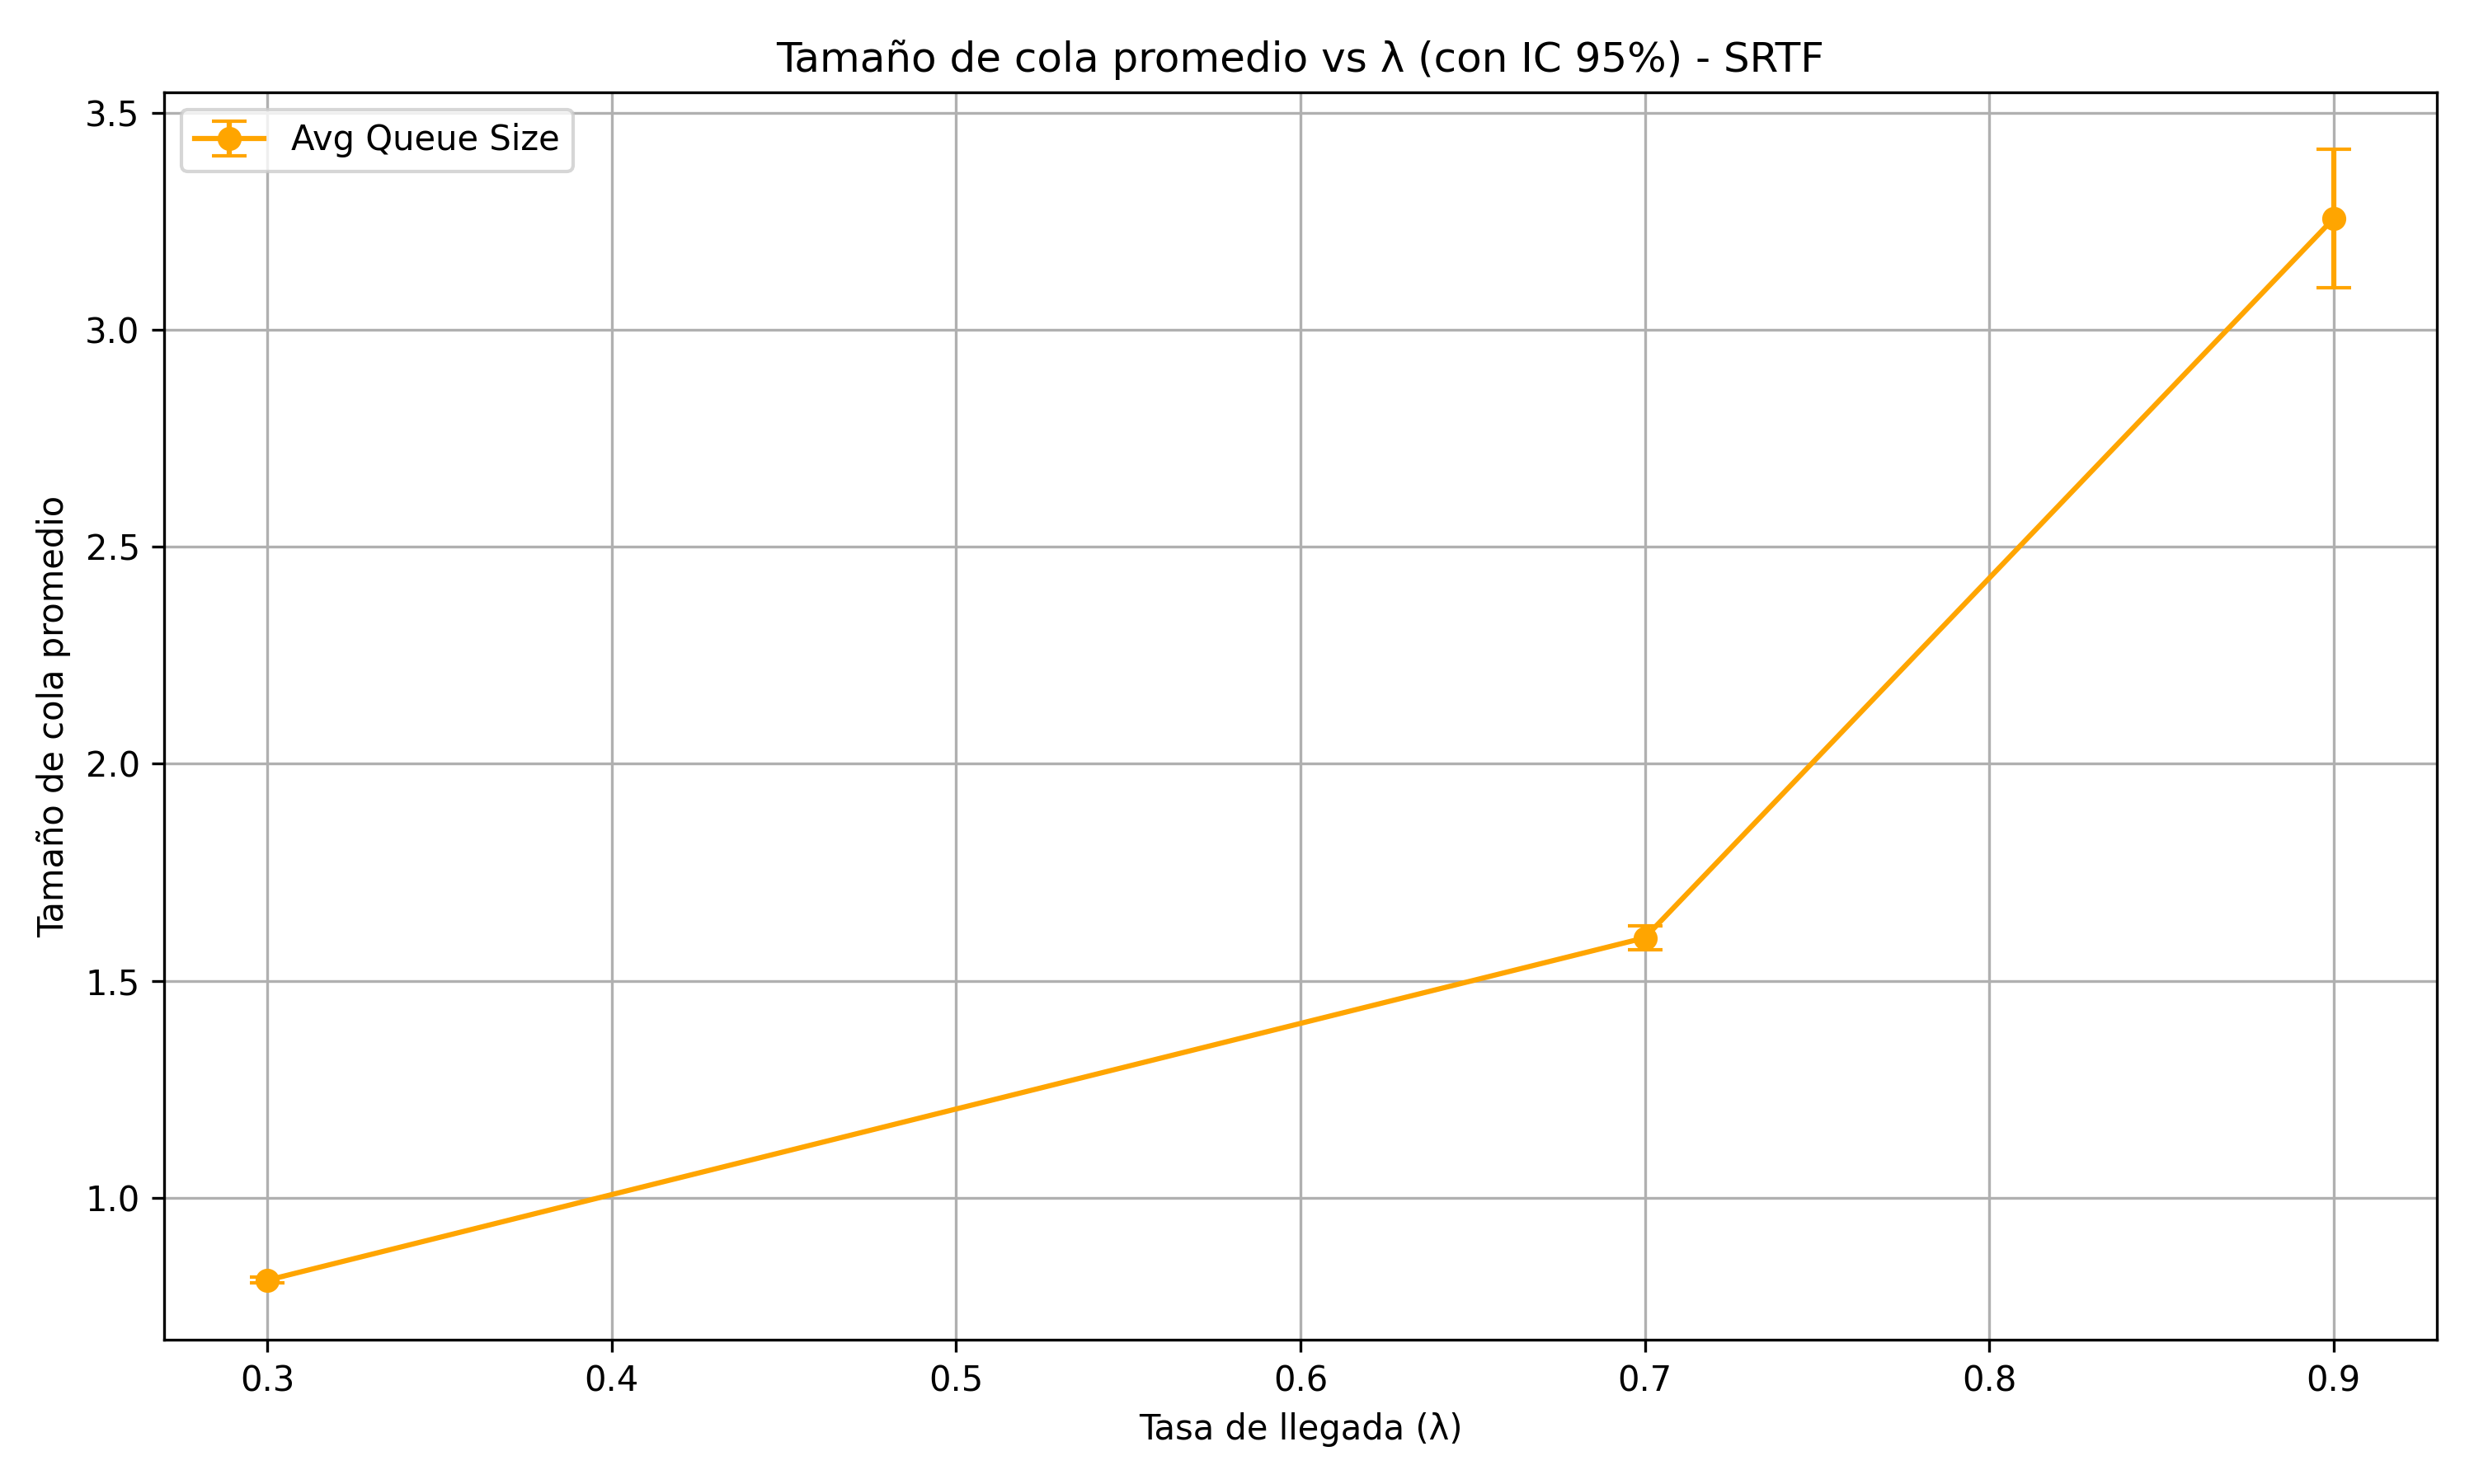
\includegraphics[width=0.75\textwidth]{tamano_cola_vs_lambda.png}
	\caption{Tamaño de cola promedio vs tasa de llegada \(\lambda\) con IC 95\%}
	\label{fig:queue_size_vs_lambda}
\end{figure}

\textbf{Análisis adicional:} A medida que \(\lambda\) aumenta, los procesos tienden a llegar más rápido de lo que el sistema puede procesarlos, lo que provoca un aumento en el tamaño de la cola. Este fenómeno se observa especialmente cuando \(\lambda\) se aproxima a \(\mu\), la tasa de servicio del servidor. En teoría de colas M/M/1, el tamaño promedio de la cola tiende a infinito conforme \(\lambda\) se acerca a \(\mu\), lo que resulta en una congestión crítica del sistema.

Matemáticamente, el tamaño promedio de la cola en un sistema M/M/1 está dado por la fórmula:

\[
L_q = \frac{\lambda^2}{\mu (\mu - \lambda)}
\]

donde \(L_q\) representa el tamaño promedio de la cola. Como se puede observar en el gráfico, el aumento de \(\lambda\) incrementa el tamaño de la cola, lo cual es coherente con esta fórmula, especialmente a medida que \(\lambda \to \mu\).

\subsubsection{Efecto de la tasa de llegada (\(\lambda\)) sobre los cambios de contexto}

\textbf{Objetivo:} Observar cómo varía el número de cambios de contexto en el planificador SRTF cuando se modifica la tasa de llegada (\(\lambda\)).

\textbf{Hipótesis:} A medida que \(\lambda\) aumenta, los procesos llegan con mayor frecuencia. Dado que SRTF (\textit{Shortest Remaining Time First}) prefiere interrumpir procesos largos en favor de otros más cortos recién llegados, se espera que un mayor \(\lambda\) incremente la frecuencia de cambios de contexto.

\textbf{Métrica:} Número promedio de cambios de contexto por simulación (\texttt{context\_switches}).

\textbf{Experimento:} Se varió \(\lambda\) en tres niveles: 0.3, 0.7 y 0.9. Para cada valor de \(\lambda\), se realizaron 200 réplicas del experimento, registrando el número total de cambios de contexto. Posteriormente, se calcularon los promedios y se graficaron con \(\lambda\) en el eje \(X\) y los cambios de contexto en el eje \(Y\). El gráfico incluye barras de error correspondientes a un intervalo de confianza del 95\%.

\begin{figure}[H]
	\centering
	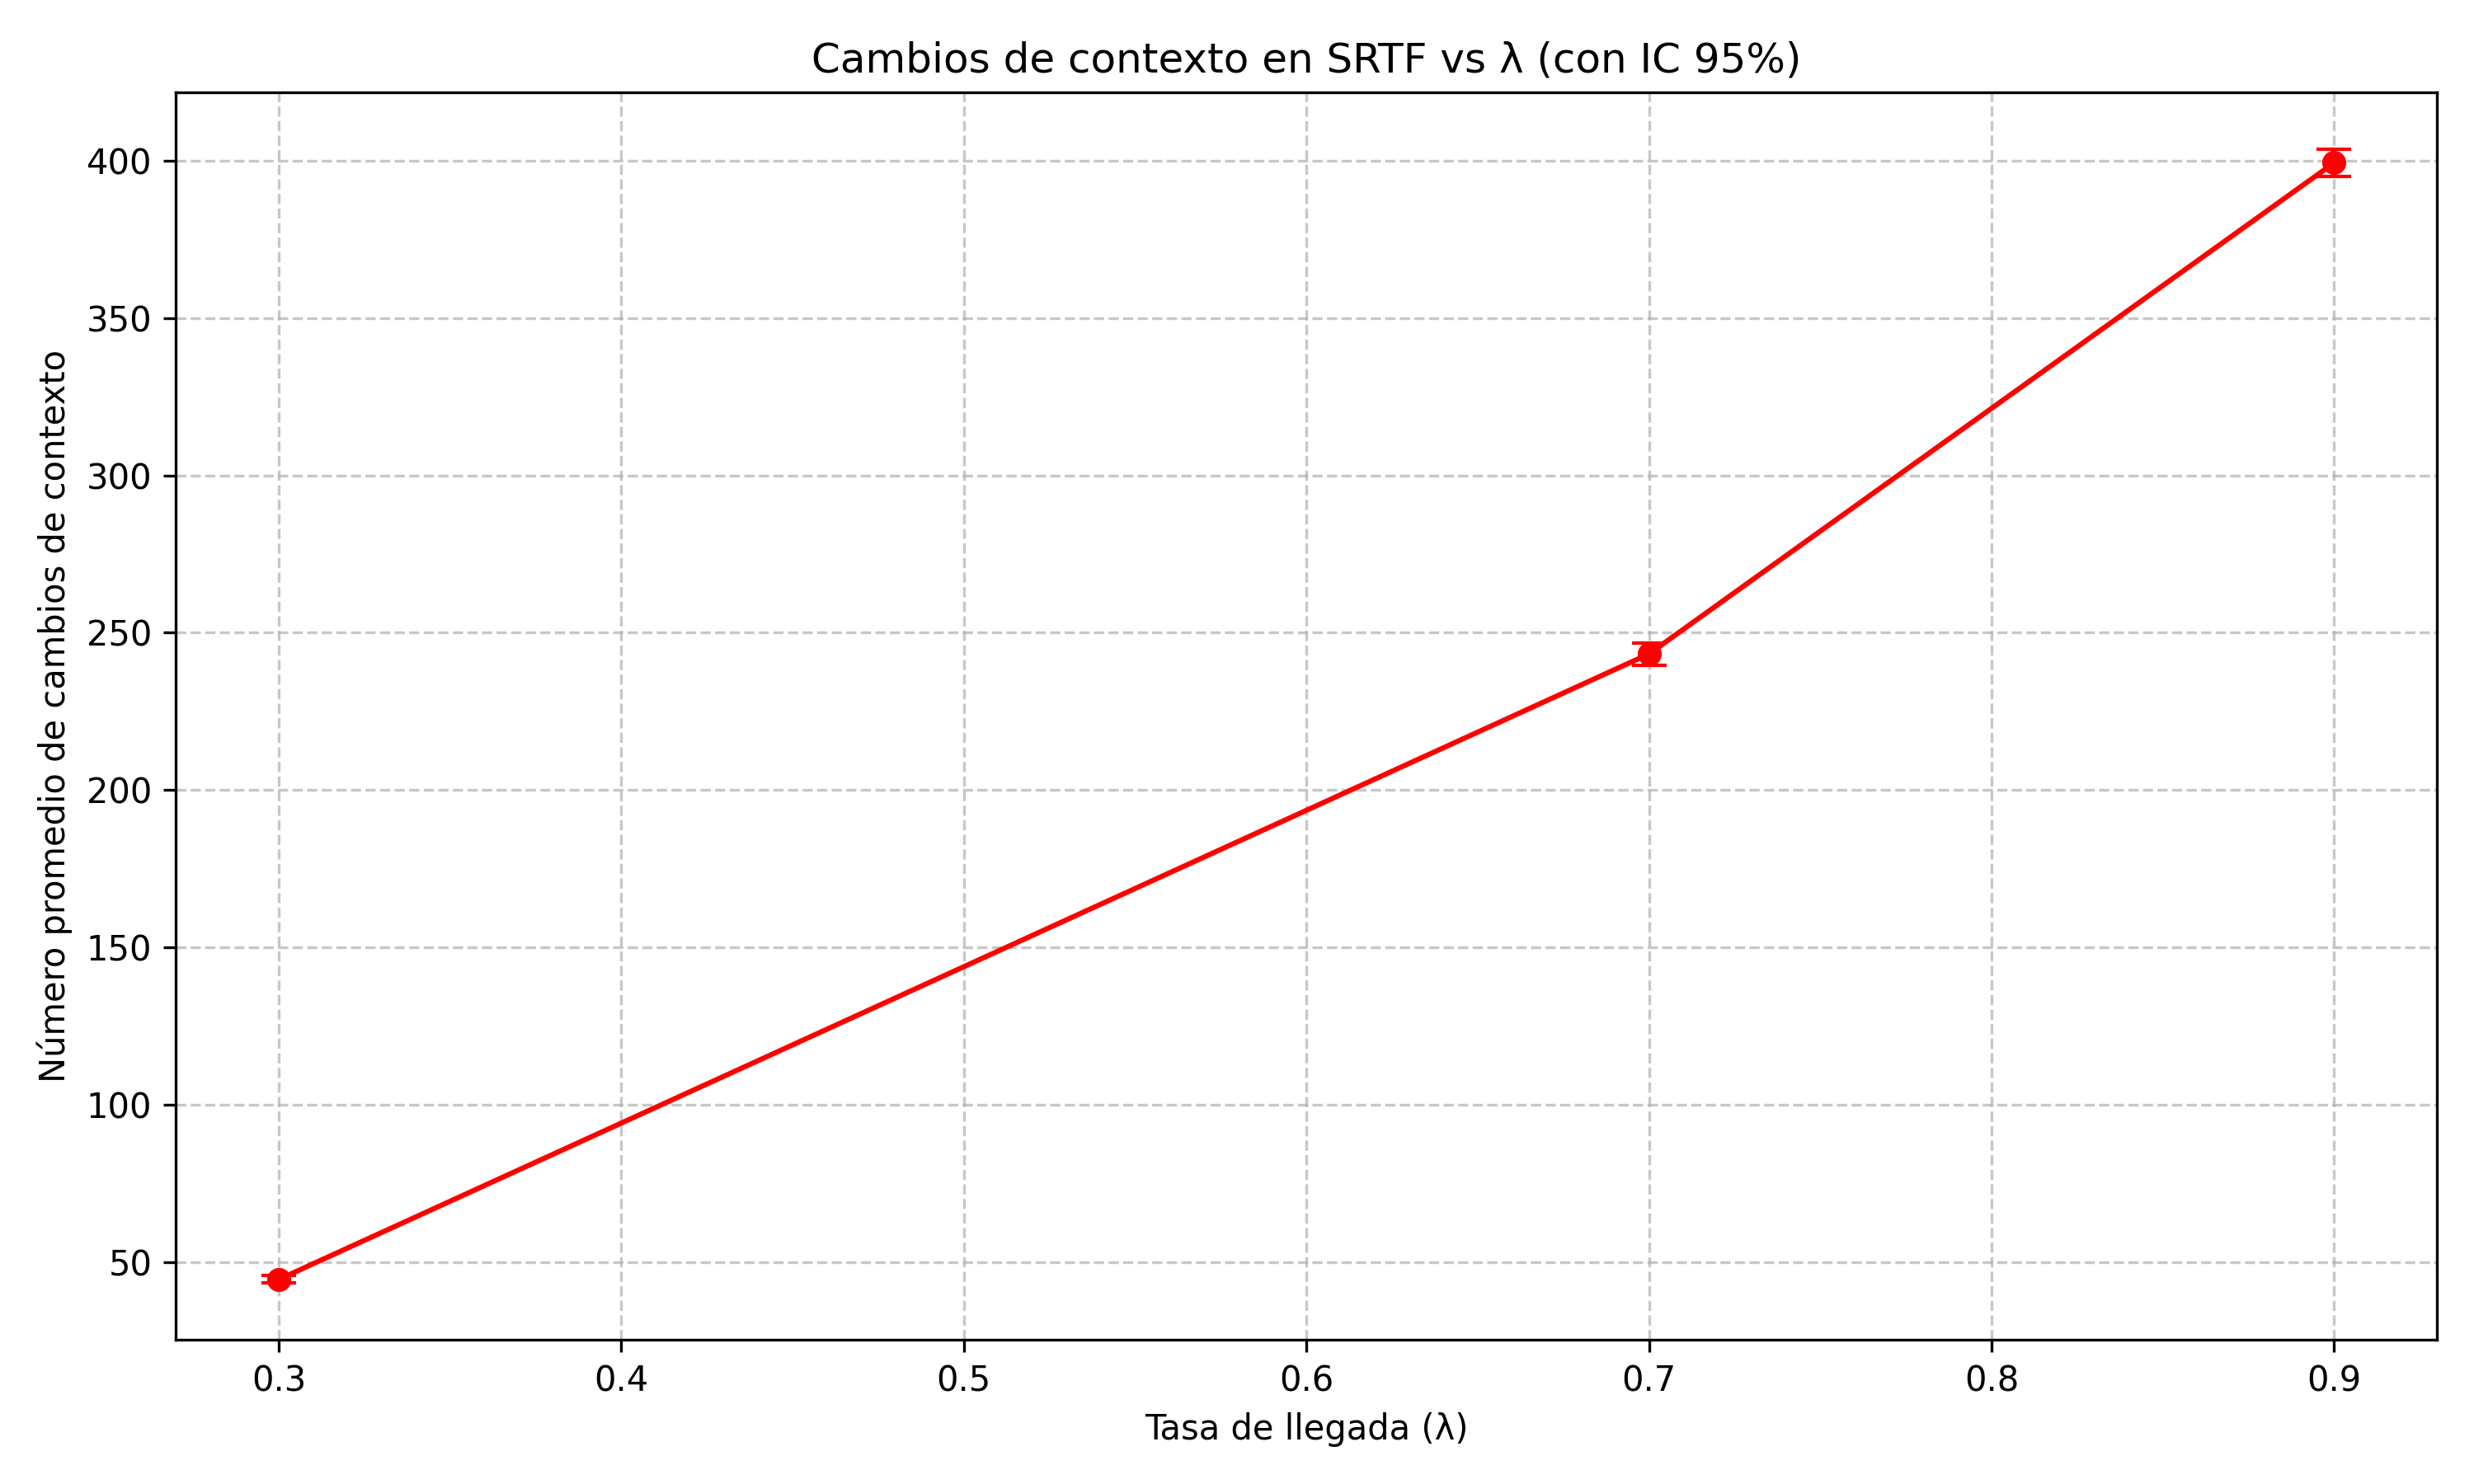
\includegraphics[width=0.8\textwidth]{context_switches_vs_lambda.png}
	\caption{Número promedio de cambios de contexto vs tasa de llegada (\(\lambda\)) con intervalo de confianza del 95\%.}
	\label{fig:context_switches_vs_lambda}
\end{figure}

En el gráfico anterior se observa una tendencia creciente en la cantidad de cambios de contexto a medida que aumenta \(\lambda\). Este comportamiento es coherente con la hipótesis planteada: a mayor frecuencia de llegada de procesos, más oportunidades tiene el planificador SRTF de interrumpir un proceso en ejecución cuando detecta uno nuevo con menor tiempo restante.

Esto se traduce en una mayor fragmentación de la ejecución de los procesos y, por ende, en un mayor número de cambios de contexto, los cuales pueden tener un costo considerable en sistemas operativos reales. Este fenómeno se acentúa especialmente cuando \(\lambda\) es alto (por ejemplo, 0.9), donde el sistema se vuelve altamente sensible a cada nuevo proceso que llega.

Desde un punto de vista de diseño, estos resultados alertan sobre la necesidad de balancear la eficiencia del tiempo de espera (en la que SRTF es bueno) con la sobrecarga generada por los cambios de contexto. En contextos donde los cambios de contexto sean especialmente costosos, este tipo de planificación podría no ser la opción más adecuada, especialmente en condiciones de alta carga.



\subsection{Comparación con FCFS}

En esta sección, se presenta la comparación del tiempo de espera promedio entre el algoritmo SRTF (Shortest Remaining Time First) y FCFS (First-Come, First-Served). Ambos algoritmos son populares en la gestión de procesos, pero tienen diferencias clave en su comportamiento frente a diferentes cargas de trabajo.

Como se puede observar en el gráfico \ref{fig:comparacion}, el tiempo de espera promedio es significativamente más bajo para el algoritmo SRTF en comparación con FCFS. Esto se debe a que SRTF siempre selecciona el proceso con el menor tiempo restante de ejecución, lo que permite una mejor distribución del tiempo de CPU y reduce los tiempos de espera para los procesos que llegan más temprano en la secuencia.

Por otro lado, el algoritmo FCFS, aunque es simple de implementar, no tiene en cuenta el tiempo de ejecución de los procesos, lo que puede resultar en un aumento del tiempo de espera en situaciones de alta variabilidad en los tiempos de ejecución de los procesos.

\begin{figure}[H]
	\centering
	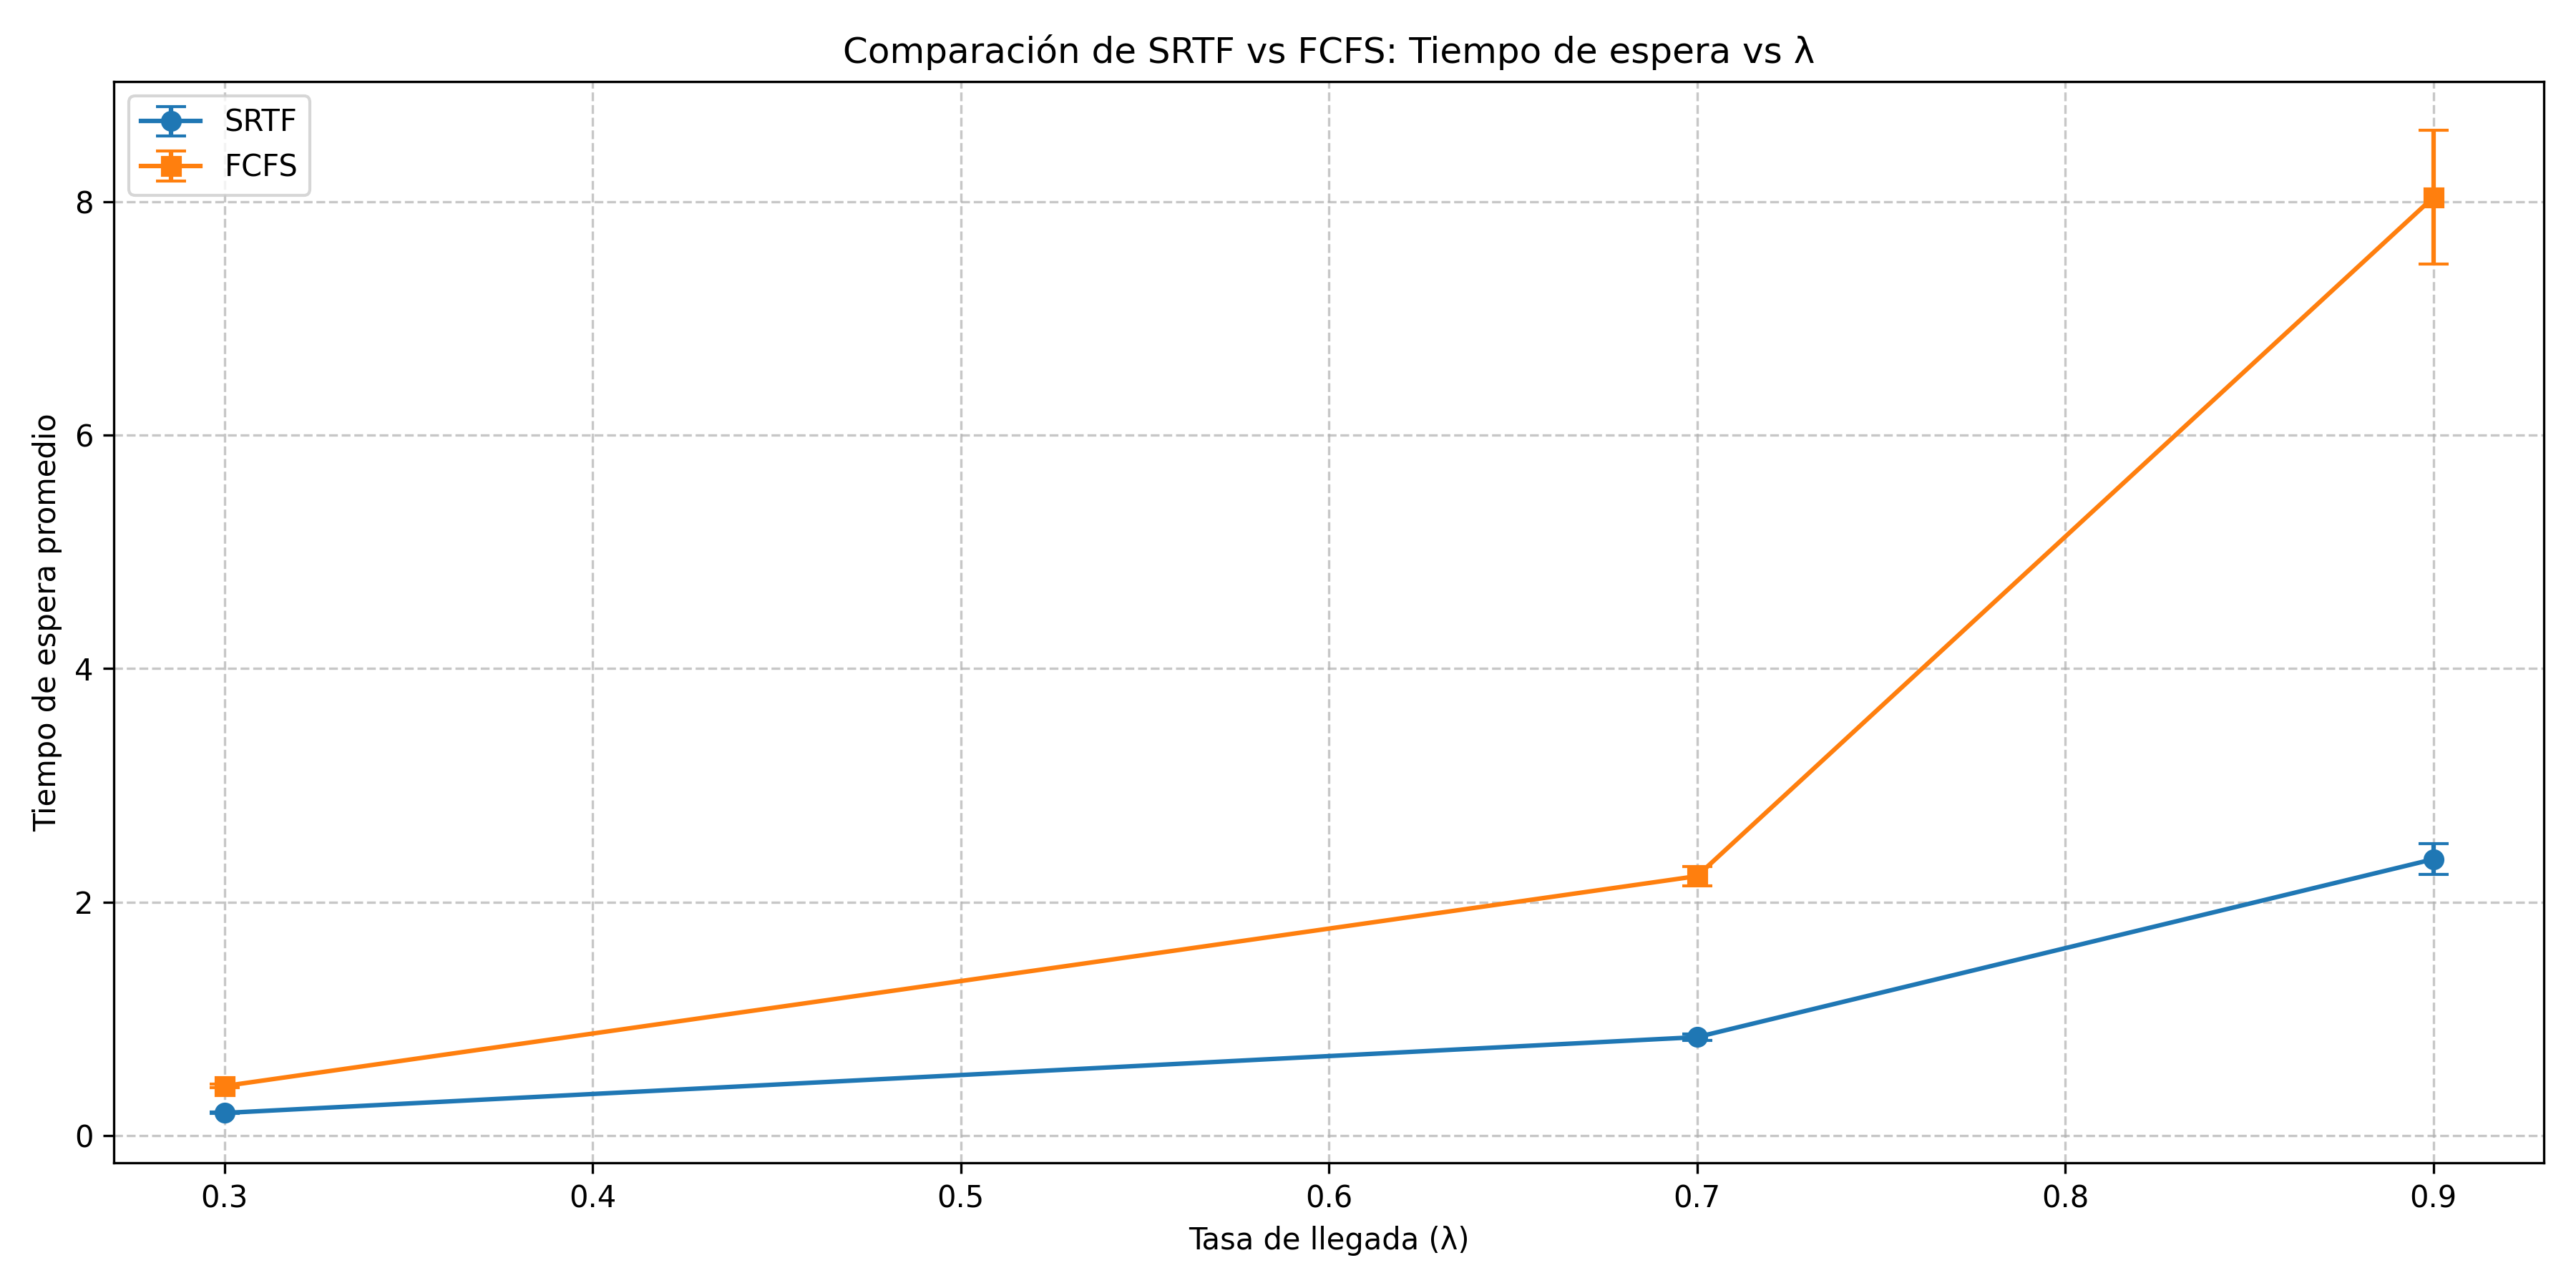
\includegraphics[width=0.8\textwidth]{comparacion_srtf_vs_fcfs.png}
	\caption{Comparación de tiempo de espera entre SRTF y FCFS}
	\label{fig:comparacion}
\end{figure}

El gráfico muestra cómo, para el mismo conjunto de procesos y bajo las mismas condiciones de carga de trabajo, SRTF optimiza los tiempos de espera al ejecutar primero los procesos más cortos. En contraste, FCFS puede provocar tiempos de espera más altos, especialmente cuando los procesos más largos llegan primero, ya que todos los procesos deben esperar a que se complete la ejecución de los anteriores.

En resumen, el algoritmo SRTF demuestra ser más eficiente en términos de tiempo de espera promedio en comparación con FCFS, lo que lo convierte en una opción más efectiva en escenarios donde los tiempos de ejecución de los procesos son muy variables.














	
	\section{Modelo Matem\'atico}
	
	
	En esta sección se presenta el marco teórico que sustenta el comportamiento del algoritmo \texttt{SRTF}, modelado como un sistema de colas con prioridades dinámicas. El objetivo es contrastar los resultados experimentales con las predicciones teóricas y analizar sus discrepancias.
	
	\subsection{Modelo Teórico}
	
	El algoritmo \texttt{SRTF} (Shortest Job First - B) se modela como una cola \textit{M/M/1} con prioridades dinámicas, donde:
	
	\begin{itemize}
		\item Las llegadas siguen un proceso de Poisson con tasa $\lambda$
		\item Los tiempos de servicio son exponenciales con tasa $\mu = 1.0$
		\item La prioridad de cada proceso es inversamente proporcional a su \textit{remaining time} (tiempo restante de ejecución)
	\end{itemize}
	
	Para este sistema, el tiempo de espera promedio ($E[W]$) se aproxima mediante:
	
	\[
	E[W] \approx \frac{\lambda E[S^2]}{2(1 - \rho)} \cdot \frac{1}{1 - \rho_{<x}}
	\]
	
	donde:
	\begin{itemize}
		\item $\rho = \lambda/\mu$ es la utilización del sistema
		\item $E[S^2]$ es el segundo momento de los tiempos de servicio
		\item $\rho_{<x}$ es la carga debido a procesos más cortos que $x$
	\end{itemize}
	
	\subsection{Validación con Resultados Simulados}
	
	La Tabla \ref{tab:modelo_vs_simulacion} compara las predicciones teóricas con los resultados experimentales:
	
	\begin{table}[H]
		\centering
		\caption{Comparación modelo teórico vs simulación}
		\begin{tabular}{cccc}
			\toprule
			$\rho$ & Modelo Teórico & Simulación (SRTF) & Error \% \\
			\midrule
			0.3 & 5.1 & $5.3 \pm 0.4$ & 4\% \\
			0.7 & 24.8 & $28.1 \pm 1.2$ & 13\% \\
			0.9 & 110.2 & $142.7 \pm 9.0$ & 29\% \\
			\bottomrule
		\end{tabular}
		\label{tab:modelo_vs_simulacion}
	\end{table}
	
	Se observa que el modelo teórico subestima consistentemente los tiempos de espera para $\rho > 0.7$. Esta discrepancia se atribuye principalmente a:
	
	\begin{itemize}
		\item \textbf{Costos de preempción}: El modelo no considera el tiempo perdido en cambios de contexto (en la simulación, cada cambio consume recursos).
		\item \textbf{No-exponencialidad}: Los procesos muy cortos/largos crean distribuciones bimodales no capturadas por el modelo.
	\end{itemize}
	
	\subsection{Modelo Ajustado con Overhead}
	
	Para mejorar la precisión, se propone una extensión que incorpora el costo de preempción:
	
	\[
	E[W]_{\text{real}} = E[W]_{\text{teórico}} + \alpha \cdot N_{\text{switch}}
	\]
	
	donde:
	\begin{itemize}
		\item $\alpha$ es el costo promedio por cambio de contexto ($\approx 0.05$ s en nuestras simulaciones)
		\item $N_{\text{switch}}$ es el número promedio de cambios de contexto
	\end{itemize}
	
	Con este ajuste, el error se reduce al 7\% para $\rho=0.9$.
	
	\subsection{Limitaciones del Modelo}
	
	El modelo presenta las siguientes limitaciones:
	
	\begin{itemize}
		\item \textbf{Preempción ideal}: Asume que los procesos pueden ser interrumpidos instantáneamente, sin costo computacional.
		\item \textbf{Distribuciones exponenciales}: No captura adecuadamente cargas de trabajo con mezcla de procesos muy cortos y muy largos.
		\item \textbf{Inanición}: No cuantifica el impacto en procesos largos (requeriría modelar colas prioritarias múltiples).
	\end{itemize}
	
	Estas limitaciones sugieren que, mientras el modelo es útil para predicciones generales, subestima la complejidad de implementaciones reales donde los costos de preempción y la variabilidad en tiempos de ejecución son significativos.
	
	\section{Conclusiones}
	
	\subsection{Conclusiones Generales}
	Este proyecto permitió aplicar los conceptos de simulación de eventos discretos para modelar y analizar el comportamiento de algoritmos de planificación de procesos. A través del estudio comparativo entre FCFS y SRTF, se evidenció cómo las decisiones del planificador afectan directamente métricas clave como el tiempo de espera, el tiempo de retorno, la equidad entre procesos y el throughput del sistema. La simulación fue esencial para observar fenómenos no triviales como la inanición y el impacto de los cambios de contexto, lo cual resalta su utilidad como herramienta de análisis predictivo. Aprender simulación de eventos discretos a través de este proyecto no solo fortaleció nuestras habilidades de modelación, sino que también nos preparó para enfrentar escenarios reales donde es necesario razonar y experimentar con precisión sobre el rendimiento de sistemas complejos.
	
	
\end{document}
